%\documentclass{sig-alternate}
\documentclass{vldb}
\usepackage{url}
%\usepackage{algorithm}
%\usepackage{algorithmic}
%\usepackage{minted}
\usepackage{subfigure}
% \usepackage[total={6.5in,9in}, top=1.25in,left=0.9in]{geometry}
%\usepackage[text={6.5in,9in},centerpage,includefoot]{geometry}
% \usepackage{setspace}
\usepackage{color}
\usepackage{url}
\usepackage{balance}

\definecolor{grey}{RGB}{200,200,200}
\newcommand{\hilite}[1]{\colorbox{grey}{#1}}
\newcommand{\hilitey}[1]{\colorbox{yellow}{#1}}
\newcommand{\hiliting}[1]{\colorbox{grey}{#1}}
\newcommand{\INDSTATE}[1][1]{\STATE\hspace{#1\algorithmicindent}}
\long\def\todo#1{\hilitey{{\bf TODO:} {\em #1}}}
\long\def\shorten#1{}
\def\azdb{\hbox{\sc AZDBLab}}
%\def\azdb{\hbox{\sc DBLab}}
\def\QatC{Q{@}C}
\long\def\comment#1{}
%c2j: Conference to Journal: first parameter is conference, second is journal
% For Conferences: c2j#1#2{#1}
% For Journals: c2j#1#2{2}
\long\def\c2j#1#2{#1}
 
%\conferenceinfo{SIGMOD'14,} {June 22--27, 2014, Salt Lake City, Utah, USA.}
%\CopyrightYear{2014}
%\crdata{978-1-4503-2037-5/13/06}
%\clubpenalty=10000
%\widowpenalty = 10000

\begin{document}
\pagenumbering{gobble}

%don't want date printed
\date{}

%make title bold and 14 pt font (Latex default is non-bold, 16 pt)
%\title{A Laboratory Information System for Empirical Studies on a Variety of DBMSes}
\title{AZDBLab: A Laboratory Information System for Large-Scale Empirical DBMS Studies}
%\numberofauthors{1}
%\author{
% DRAFT
%}
%
\numberofauthors{3}
\author{
%
% The command \alignauthor (no curly braces needed) should
% precede each author name, affiliation/snail-mail address and
% e-mail address. Additionally, tag each line of
% affiliation/address with \affaddr, and tag the
%% e-mail address with \email.
% 1st author
\alignauthor
Young-Kyoon Suh\\
%       \affaddr{Department of Computer Science}\\
       \affaddr{University of Arizona}\\
%       \affaddr{Tucson, AZ}\\ 
       \affaddr{\small\tt yksuh@cs.arizona.edu}
%2nd author
\alignauthor
Richard T.~Snodgrass\\
%       \affaddr{Department of Computer Science}\\
       \affaddr{University of Arizona}\\
%       \affaddr{Tucson, AZ}\\
       \affaddr{\small\tt rts@cs.arizona.edu}
%3rd author
%\alignauthor
%Rui Zhang\\
%       \affaddr{Dataware Ventures}\\
%%       \affaddr{Torrence, CA}\\
%       \email{\small\tt ruizhang@datawareventures.com}
\alignauthor
Rui Zhang\\
%       \affaddr{Department of Computer Science}\\
       \affaddr{Dataware Ventures}\\
%       \affaddr{Tucson, AZ}\\
       \affaddr{\small\tt ruizhang@datawareventures.com}
\shorten{
\and 
%%4th author
\alignauthor
Matthew Wong Johnson\\
%      \affaddr{Department of Computer Science}\\
       \affaddr{Univ. of California, San Diego}\\
%       \affaddr{San Diego, CA}\\
       \email{\small\tt mwj@email.arizona.edu}
%%%5th author
\alignauthor
Andrey Kvochko\\
%       \affaddr{Department of Computer Science}\\
       \affaddr{University of Arizona}\\
%       \affaddr{Tucson, AZ}\\
       \affaddr{\small\tt akvochko@cs.arizona.edu}
%6th author
\alignauthor
Benjamin Dicken\\
%       \affaddr{Department of Computer Science}\\
       \affaddr{University of Arizona}\\
%       \affaddr{Tucson, AZ}\\
       \affaddr{\small\tt bddicken@cs.arizona.edu}
}
}
%\date{%\vspace*{-1cm}}

\maketitle
%\vspace*{-3in}

\begin{abstract}%\todo{Young: Rewrite this after finalizing body.} 
%Understanding a variety of behaviors present in DBMSes 
%can give an importance implication database query optimizers to improve. 
%There has been no system to study these aspects across different DBMSes. 
%This scientific approach leads to fundamental improvements 
%of database query optimizers. 
%To address this ,
%There has been no system of allowing database researchers to 
%simultaneously run experiments on different DBMSes and seamlessly analyze the results, 
%to better understand a variety of behaviours of database query optimizers. 

%In database field, scientific approach has been much less prominent while very strong 
%mathematical and engineering work has been done. 
%Understanding database query optimizers better, for instance, is of critical importance, 
%as it can provide great insights into their improvements by looming 
%which parts should be re-examined. 
%However, there has been few systems for supporting such a scientific approach.

In the database field, while very strong 
mathematical and engineering work has been done, the 
scientific approach has been much less prominent. 
\shorten{Understanding database query optimizers better, for instance, is of critical importance, 
as it can provide insights into their improvements by \hbox{identifying} which parts should be re-examined.}
The deep understanding of query optimizers obtained through the scientific approach can lead to better engineered designs.
Unlike other domains, there have been few {\em DBMS-dedicated} laboratories, 
focusing on such scientific investigation. 

%In this demonstration, we present a novel laboratory information system, 
%called {\em Arizona Database Laboratory} ($\azdb$), to assist database researchers 
%to empirically study DBMSes in a scientific manner. 
%For one to test their hypotheses on the behavior of query optimizers, 
%our system can allow him or her to simultaneously run and monitor a variety of experiments on multiple DBMSes. 
%Furthermore, the system can later automatically analyze the results. 
%The audience will interact with $\azdb$ through the stand-alone 
%application or the mobile app to get to conduct an experiment. 
%Subsequently, the audience will visually 
%see the analysis results on the completed experiment in the form of a paper.

In this demonstration, we present a novel DBMS-oriented research infrastructure, 
called {\em Arizona Database Laboratory} \linebreak ($\azdb$), to assist database researchers 
in conducting a {\em large-scale} empirical study across multiple \hbox{DBMSes}\shorten{ in a {\em scientific} manner}. 
For them to test their hypotheses on the behavior of query \linebreak \hbox{optimizers}, 
$\azdb$ can run and monitor a large-scale \hbox{experiment} with thousands (or millions) of queries on \linebreak \hbox{different} \hbox{DBMSes}. 
Furthermore, $\azdb$ can help users \linebreak \hbox{automatically} analyze these queries. 
In the demo, the \linebreak \hbox{audience} will interact with $\azdb$ through the stand-alone
\hbox{application} and the mobile app to conduct such a large-scale \hbox{experiment} for a study. 
The \hbox{audience}  will then run a Tucson \hbox{Timing} \hbox{Protocol} analysis on the finished \linebreak \hbox{experiment} and then see the analysis (data sanity check and timing) \hbox{results}. 

%
%Understanding database query optimizers is of critical importance in a sense that it can provide 
%great insights into what parts of the optimizers should be examined for their improvements. 
%However, this scientific approach has been much less prominent in database field while very stong 
%mathematical and engineering work has been done. 
%For instance, there has been no system of allowing database researchers to 
%simultaneously run experiments on different DBMSes and seamlessly analyze the results. 
%To support this scientific, empirical study on DBMSes, in this paper we introduce a novel laboratory information system, 
%called {\em Arizona Database Laboratory} ($\azdb$). 
\end{abstract}

% A category with the (minimum) three required fields
%\category{H.4}{Information Systems Applications}{Miscellaneous}
%A category including the fourth, optional field follows...
%\category{D.2.8}{Software Engineering}{Metrics}[complexity measures, performance measures]

\section{Introduction}\label{sec:intro}
%Understanding database query optimizers is of critical importance in a sense that it can provide 
%great insights into what parts of the optimizers should be examined for their improvements. 
%Also, it can ultimately derive predictive theories about how optimizers as a general class behave, which will be very 
%useful in the enhanced design of query optimizers. 
%Despite these strengths, this scientific approach has been much less prominent in database field while very stong 
%mathematical and engineering work has been done. 
%For instance, there has been no system of allowing database researchers to 
%simultaneously run experiments on different DBMSes and seamlessly analyze the results. 
%To support this scientific, empirical study on DBMSes, we introduce a novel laboratory information system, 
%called {\em Arizona Database Laboratory} ($\azdb$). 
%In database field, scientific approach has been much less prominent while very strong 
%engineering and mathematical work has been done. 
In the database field, while very strong mathematical and engineering work has been done, the 
scientific approach has been much less prominent. 
Much work has focused on \linebreak \hbox{proposing} new algorithms for optimizing DBMS performance 
and on building system components for new needs, but the \hbox{community} has not devoted 
much attention on \hbox{scientifically} understanding \hbox{DBMS} as an {\em experiment subject}. 
\shorten{\hbox{Indeed}, understanding database query optimizers better is of critical importance, 
as it can provide insights into their improvements by identifying which parts should be re-examined. 
Also, it can ultimately derive predictive theories about the database optimizer behavior, 
thereby leading to their enhanced designs.} 
The deep understanding of query optimizers obtained through the \linebreak \hbox{scientific} approach 
can lead to better engineered designs.

There, however, have been few {\em DBMS-dedicated} \linebreak \hbox{laboratories}
for supporting such \hbox{scientific} \hbox{investigation}, while prior work mainly has focused on 
%networks ({\it e.g.,} 
%\hbox{PlanetLab}~\cite{Peterson2006planetlab}\shorten{\footnote{http://www.planet-lab.org/}}), 
%\hbox{sensors} ({\it e.g.,} 
%\hbox{MoteLab}~\cite{WA05MoteLab}\shorten{\footnote{http://motelab.eecs.harvard.edu/}}), 
%\hbox{smartphones} ({\it e.g.,} 
%\hbox{SmartLab}~\cite{Larkou13SmartLab}\shorten{\footnote{http://smartlab.cs.ucy.ac.cy/}}, 
%\hbox{PhoneLab}~\cite{Nandugudi13PhoneLab}\shorten{\footnote{http://www.phone-lab.org/}}, 
%\hbox{CrowdLab}~\cite{cuervo2011crowdlab}), 
%{\it etc}. 
\hbox{networks} and smartphones as we will discuss in Section~\ref{sec:related_work}.

In this demonstration, we present a novel DBMS-oriented \hbox{research} infrastructure, 
called {\em Arizona Database Laboratory} ($\azdb$), to assist database researchers 
to conduct a {\em large-scale} empirical study across {\em multiple} \hbox{DBMSes}\shorten{ in a {\em scientific} manner}. 

$\azdb$ presents to a scientist an electronic lab \linebreak \hbox{notebook}. 
Within this environment, the user can \hbox{design} massive \hbox{experiments} with \hbox{thousands} (or millions) of queries. 
%(Running TPC benchmarks within $\azdb$ is not yet considered, but it will be possible in the future.)
The user can then begin and monitor many runs of the \hbox{experiments} \shorten{tens (or hundreds or more)} 
on different \hbox{DBMSes} over a long period of time. 

In addition, $\azdb$ provides an integrated and robust database experiment environment. 
In $\azdb$, a user can record both independent variables (those controlled by the \hbox{experimenter}) 
and dependent variables (those \hbox{resulting} from the \hbox{experiment}) and perform analyses on the \linebreak \hbox{experiment} data. 
For instance, the user can easily \hbox{combine} the \hbox{completed} runs in a study and then analyze in an \linebreak \hbox{automated} way for the study the query execution (QE) \linebreak \hbox{results}. 
\shorten{Note that every query at a given cardinality gets executed 10 times, and each QE \hbox{result} contains not only QE-specific \hbox{information} (query plan and measured time) but also the \hbox{compressed} detailed \hbox{information} of \hbox{approximately} two \hbox{hundred} processes per QE in those runs. (The raw QE \hbox{result} size is about 568KB, but when compressed, it is \hbox{reduced} to \hbox{approximately} 32KB.)}
In addition, \hbox{$\azdb$} has been sufficiently \hbox{robust} to collect data over 8,277 hours (\hbox{almost} a year) 
running about 2.4 million query executions. 

%$\azdb$ consists of about 60K source lines of code and currently supports experiments on seven \hbox{DBMSes}, 
%four commercial and three open-source. 
%To the scientist, $\azdb$ presents an electronic laboratory notebook. 
%Within this environment, one can design and specify experiments, 
%schedule these experiments, monitor them when they are running, 
%record both independent variables (those controlled by the experimenter) and 
%dependent variables (those \hbox{resulting} from the experiment) and perform analyses on the data. 
%\hbox{$\azdb$} runs on a hardware lab of dedicated machines, 
%one each for each subject DBMS and one to host the DBMS that stores the lab notebooks, called {\em labshelves}. 
%%Having dedicated hardware allows us to worry less about other processes running on the machines 
%%that could dirty the results (these machines are only for experiments), and allows us to run extensive 
%%experiments taking days or weeks. 
%Having dedicated hardware provides a clear environment and allows us to run extensive experiments taking days or weeks.

The design and implementation of $\azdb$ has been very challenging. 
$\azdb$ has been developed for seven years by many people, each contributing to different pieces of code. 
\shorten{As of March 20, 2014,} $\azdb$ has reached 60K source lines of code. 
\hbox{$\azdb$} runs on a hardware lab of dedicated machines, 
one each for each subject DBMS and one to host the DBMS that stores the lab notebooks on a {\em labshelf}. 
%Having dedicated hardware allows us to worry less about other processes running on the machines 
%that could dirty the results (these machines are only for experiments), and allows us to run extensive 
%experiments taking days or weeks. 
%Having dedicated \hbox{hardware} provides a clear environment and allows us to run extensive experiments taking days or weeks. 
Having \hbox{dedicated} \hbox{hardware} provides a clear environment for \hbox{running} large-scale, extensive experiments taking days, weeks, or months.
A total of seven relational \hbox{DBMSes} (four \hbox{commercial} and three open-source) supporting 
SQL and JDBC are \hbox{currently} integrated into $\azdb$
We will plug more \hbox{DBMSes} into $\azdb$ for more solid scientific \hbox{studies}. 
\shorten{We should say that considering that the DBMSes have different \hbox{implementations} and \hbox{distinct} \hbox{characteristics}, 
it was never easy for us to plug in these \hbox{DBMSes} to and fully work with $\azdb$.}

The key contributions of this demonstration are as follows.

\begin{itemize}
\item  We present a novel research infrastructure, $\azdb$, dedicated for a large-scale scientific DBMS study. 
\linebreak $\azdb$ provides a rigorous \hbox{abstraction} for \linebreak \hbox{empirically} \hbox{studying} across
multiple \hbox{DBMSes} \shorten{in} from a \linebreak \hbox{variety} of \hbox{perspectives} (termed {\em database ergalics}~\cite{ergalics})\shorten{, like the other laboratories actively operating in \hbox{different} domains}.

%\vspace\fill

\item $\azdb$ supports seamless {\em data provenance} \linebreak \hbox{collection} within an \hbox{empirical} DBMS study. 
A \linebreak database \hbox{researcher} can \hbox{design} and run a substantial \hbox{experiment} with many queries, 
see the query \hbox{execution} \hbox{results}, perform data \hbox{sanity} check and \hbox{analysis} and 
make tables, figures, and graphs for the study in an \hbox{automated}, \hbox{integrated} \hbox{fashion}. 
Note that the data provenance of the study is collected into a \hbox{labshelf}, 
\hbox{managed} by a \hbox{central} DBMS server. %Therefore, a user can easily keep track of how data is produced through $\azdb$. 
%$\azdb$ knows which version of a protocol is used for the analysis. 

%\item $\azdb$ supports running experiments across multiple \hbox{DBMSes} (termed {\em database ergalics}). 
%The same or different experiments can be simultaneously run on different \hbox{DBMSes} within $\azdb$. 
\item For conducting large-scale experiments, $\azdb$ \linebreak \hbox{provides} several {\em decentralized \hbox{monitoring}} \linebreak schemes: 
a stand-alone Java application (named \linebreak {\em \hbox{Observer}})\shorten{(running on a separate machine not \hbox{participating} in experiments)}, 
an {\em Ajax}~\cite{ajax} web app, and a mobile app.
\shorten{Also, she can be notified via {\em watcher} when an error or an exception occurs during experiment. 
This frees her from watching the experiments at all times.}

\item $\azdb$ provides a reusable GUI architecture. \linebreak \hbox{Observer}'s GUI consists of the {\em tree nodes} in the left-hand side and the {\em tabbed viewers} in the right-hand side. The tree nodes represent \hbox{experiment} data, while the corresponding tabbed viewers provide the detailed \hbox{information} on the selected data. 
We have adapted the \hbox{GUI} to several diverse projects.

\item $\azdb$ provides rich {\em extensibility}. A variety of \hbox{{\em plugins}} provides $\azdb$ 
with various analytics and \hbox{different} views of the collected query execution data.

%\item We introduce a novel {\em laboratory information system}, called {\em Arizona Database Laboratory} ($\azdb$), for supporting empirical studies on a variety of DBMSes. 

%\item We present various {\em plugin}s enriching the extensibility of $\azdb$. 

%\item We propose a {\em robust} methodology of running an experiment in $\azdb$. 

%\item We present the automated result analysis process incorporated into $\azdb$. 

\end{itemize}

\section{Motivation}\label{sec:motivation} 

There are questions concerning fundamental limits of \linebreak \hbox{DBMS} 
architectures that simply cannot be answered by \hbox{investigating} a single \hbox{algorithm} or even a single DBMS. 
Rather, \hbox{addressing} such questions requires the development of {\em \hbox{predictive} models across multiple \hbox{DBMSes}}. 

The objective behind this {\em scientific} approach is to \linebreak \hbox{understand} \hbox{DBMSes} 
as a {\em general} class of computational \hbox{artifacts}, 
to come up with insights and ultimately with \linebreak \hbox{predictive} models 
about how such systems, again, as a \linebreak \hbox{general} class, behave by studying multiple \hbox{DBMSes} at a time. 
These models are articulated and thoroughly tested, in order to \hbox{understand} more deeply the behavior of query \hbox{optimization} and \hbox{evaluation} across multiple \hbox{DBMSes}. 
They can be \hbox{eventually} used to improve \hbox{DBMSes} through \linebreak \hbox{engineering} efforts 
that benefit from the fundamental \linebreak \hbox{understanding} by this \hbox{perspective}. 

%$\azdb$ has been designed and developed over seven years to help us 
%reach this overarching goal: to {\em \hbox{predict} important characteristics} of \hbox{DBMSes} to determine {\em fundamental limits}.}  
$\azdb$ has been around over seven years to help us achieve this overarching goal: to {\em predict important 
\linebreak \hbox{characteristics}} of \hbox{DBMSes} to determine \hbox{{\em fundamental}} \linebreak \hbox{{\em limits}}. 
$\azdb$ allows us to perform substantial \linebreak \hbox{experiments} (with thousands or more of queries) that \linebreak \hbox{quantitatively} study these fundamental questions \hbox{concerning} many of the \hbox{components} of a \hbox{DBMS}. 
These cover (i) \linebreak \hbox{{\em cardinality}} \hbox{{\em estimation}} (identifying what affects the accuracy of \hbox{cardinality} \hbox{estimates}), 
(ii) {\em operator impact} (\hbox{characterizing} how specific types of \hbox{operators}, {\it e.g.}, join, projection, \hbox{sorting}, 
\hbox{affect} the \hbox{accuracy} of cardinality \hbox{estimates}, \hbox{execution} time estimates, and \hbox{optimal} plan selection), and 
(iii) {\em \hbox{execution} plan search space} (determining its detailed inner \hbox{structure}).

As an \hbox{experiment} tool, $\azdb$ coordinates the \linebreak \hbox{running}, data \hbox{collection} and analysis of such large-scale \linebreak \hbox{experiments}. 
It has been broadened to support \hbox{experiment} \hbox{replication}, \hbox{provenance} maintenance, more variety of 
%\linebreak \hbox{experiment} \hbox{scenarios} (to be discussed in Section~\ref{sec:observer}), and more \hbox{DBMSes}. 
\linebreak \hbox{experiment} \hbox{scenarios}, and more \hbox{DBMSes}. 

\section{Related Work}\label{sec:related_work} 

Although many labs have been established and widely used, their application domains are different from \hbox{DBMSes}. \hbox{PlanetLab}~\cite{Peterson2006planetlab} 
is known as one of the most \hbox{popular} \linebreak \hbox{platforms} for network research. It allows people to 
deploy and assess network service~\cite{Peterson2006planetlab}. 
\hbox{MoteLab}~\cite{WA05MoteLab} was a \hbox{public} 
\hbox{testbed} for wireless sensor network researchers. 
Its \hbox{service} was stopped in January 2014. 

There are also available \hbox{mobile} computing research labs: \hbox{CrowdLab}~\cite{cuervo2011crowdlab}, \hbox{SmartLab}~\cite{Larkou13SmartLab}, \shorten{\hbox{PhoneLab}~\cite{Nandugudi13PhoneLab},} etc. %%% should etc be in italic?
None of these labs are, however, \hbox{{\em DBMS-centric}}.\shorten{, and there has been few laboratories dedicated for empirically studying across DBMSes.}

One of the closest tools related to $\azdb$ is Picasso~\cite{Reddy05}.
The Picasso tool can also help study query execution plan choices of (three) 
different \hbox{DBMSes}' cost-based query \linebreak \hbox{optimizers}, by generating plan and cost diagrams for \hbox{TPC-H} queries. 
Both Picasso and $\azdb$ systems use the \linebreak ``{\tt EXPLAIN}'' \hbox{command}, to see the execution plan of a query submitted to \hbox{DBMSes}. 
%However, unlike $\azdb$, that system has no functionalities of actually executing queries and collecting the query execution provenance for further analysis. 
Unlike $\azdb$, the Picasso tool neither actually runs queries nor collects the query \hbox{execution} provenance for further \hbox{analysis}.

Using $\azdb$, our empirical \hbox{DBMS} study 
has yielded two structural causal models; one that \hbox{identifies} across four \hbox{DBMSes} some of the causes of varying query time \hbox{measures}~\cite{Currim} and one that identifies several of the causal factors of \linebreak \hbox{suboptimality}, when the DBMSes choose a wrong plan. Also, we are currently working on developing another structural causal model to explain DBMS thrashing~\cite{Thomasian93}.
\shorten{We plan to add several more \hbox{commercial} \hbox{DBMSes} and open source \hbox{DBMSes} in the future.}

%In the next section, we will present the overall \hbox{architectural} components of $\azdb$. 
%We end with an outline of the demo. 

%The scope of this investigation will be significantly broadened to consider many of the components of
%a modern DBMS, including (i) cardinality estimation (identifying what affects the accuracy of 
%cardinality estimates), (ii) operator impact (characterizing how specific types of operators-e.g., joins, projection, 
%sorting—affect the accuracy of cardinality estimates, execution time estimates, and optimal plan selection), 
%(iii) execution plan search space (determining its detailed inner structure), and (iv) transaction and 
%concurrency control (specifying how throughput and disk utilization depend on multiprogramming level, how the 
%presence of hot spots affect this interaction, and when thrashing occurs). 

\section{AZDBLab System Overview}\label{sec:architecture} 
Figure~\ref{fig:azdblab_arch} presents the architecture of $\azdb$. 
In this section, we describe each component of $\azdb$. 

\begin{figure}[htp!]
\centering
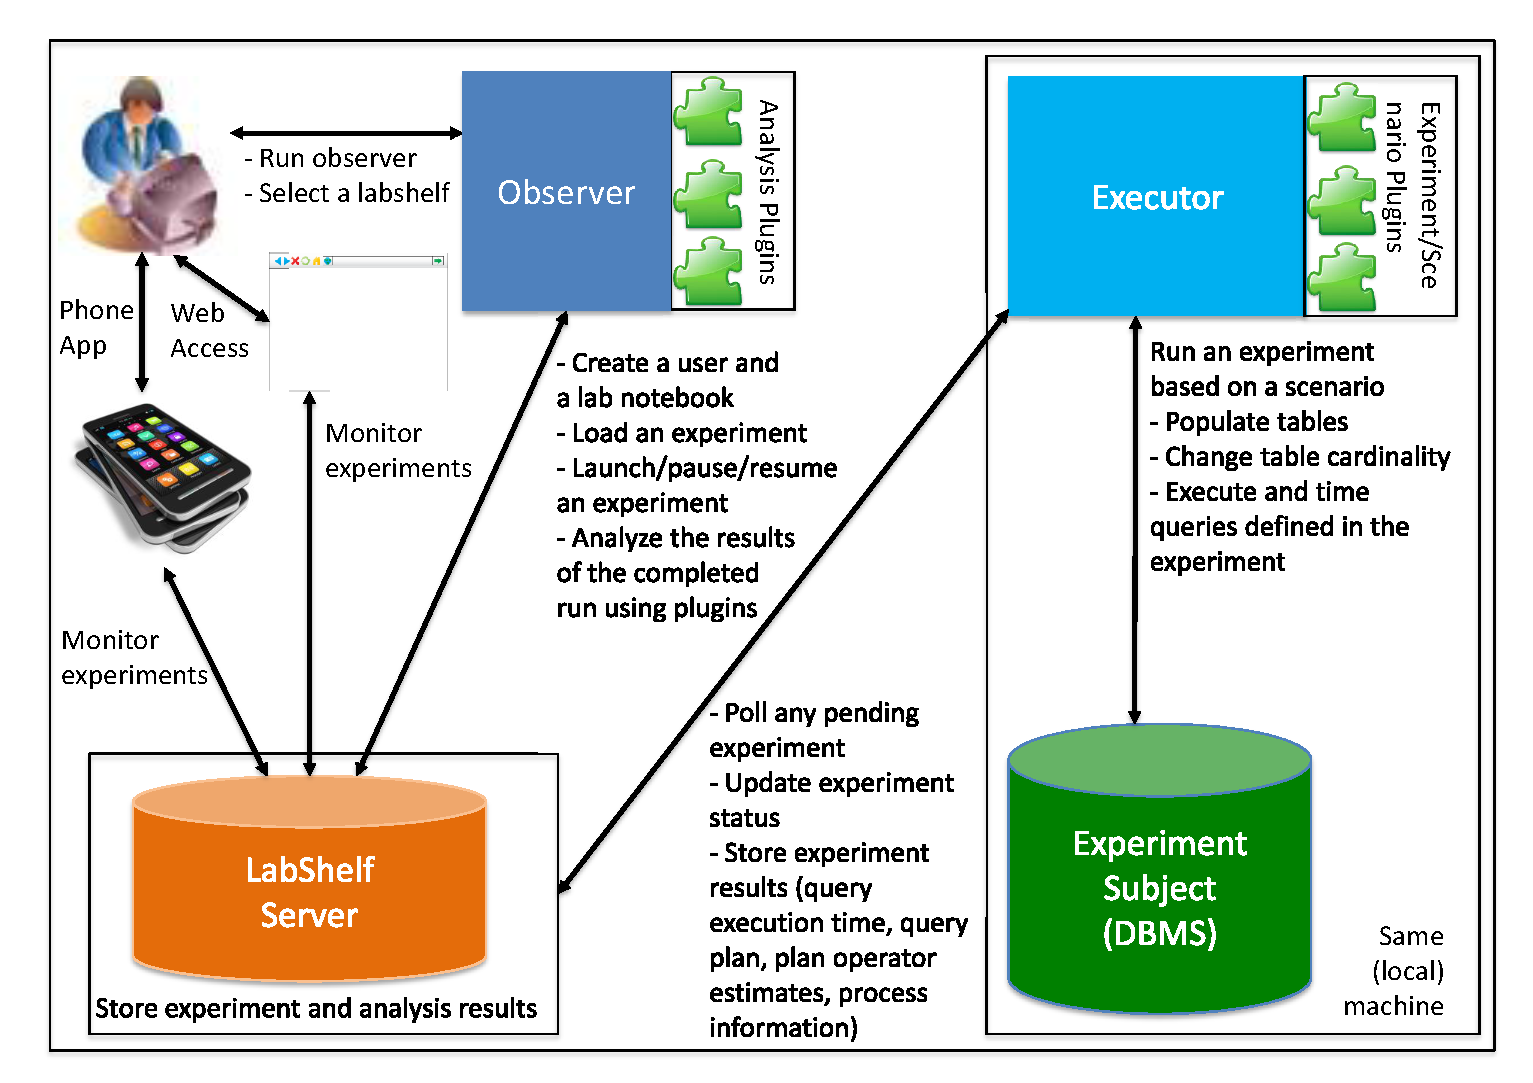
\includegraphics[scale=0.34]{./figures/azdblab_arch}
%\vspace{-0.3in}
\caption{$\azdb$ architecture~\label{fig:azdblab_arch}}
%\vspace{-0.2in}
\end{figure}

\subsection{LabShelves}
A labshelf comprehensively stores all the {\em data provenance} \hbox{related} to experiments. 
\shorten{It is created along with a {\em versioned-schema} complying with the {\em 7-W model}~\cite{Ram}.} 
It is a fully append-only database~\cite{Snodgrass99}.
The schema of a labshelf \hbox{captures} {\em who}, {\em what}, {\em when}, {\em which}, {\em where}, {\em why}, and {\em how}, \hbox{complying} with the {\em 7-W model}~\cite{Ram}. 
%That said, there is provenance that the system does not yet capture. 
The labshelf schema has been evolving for collecting and \hbox{analyzing} a \hbox{variety} of data relevant to QE.
The labshelf data are currently managed by a dedicated DBMS server \hbox{running} on a separate machine.  
\shorten{separated from machines hosting \hbox{experiment} \hbox{subjects}.}

%\vspace\fill

\begin{figure*}[htp!]
\centering
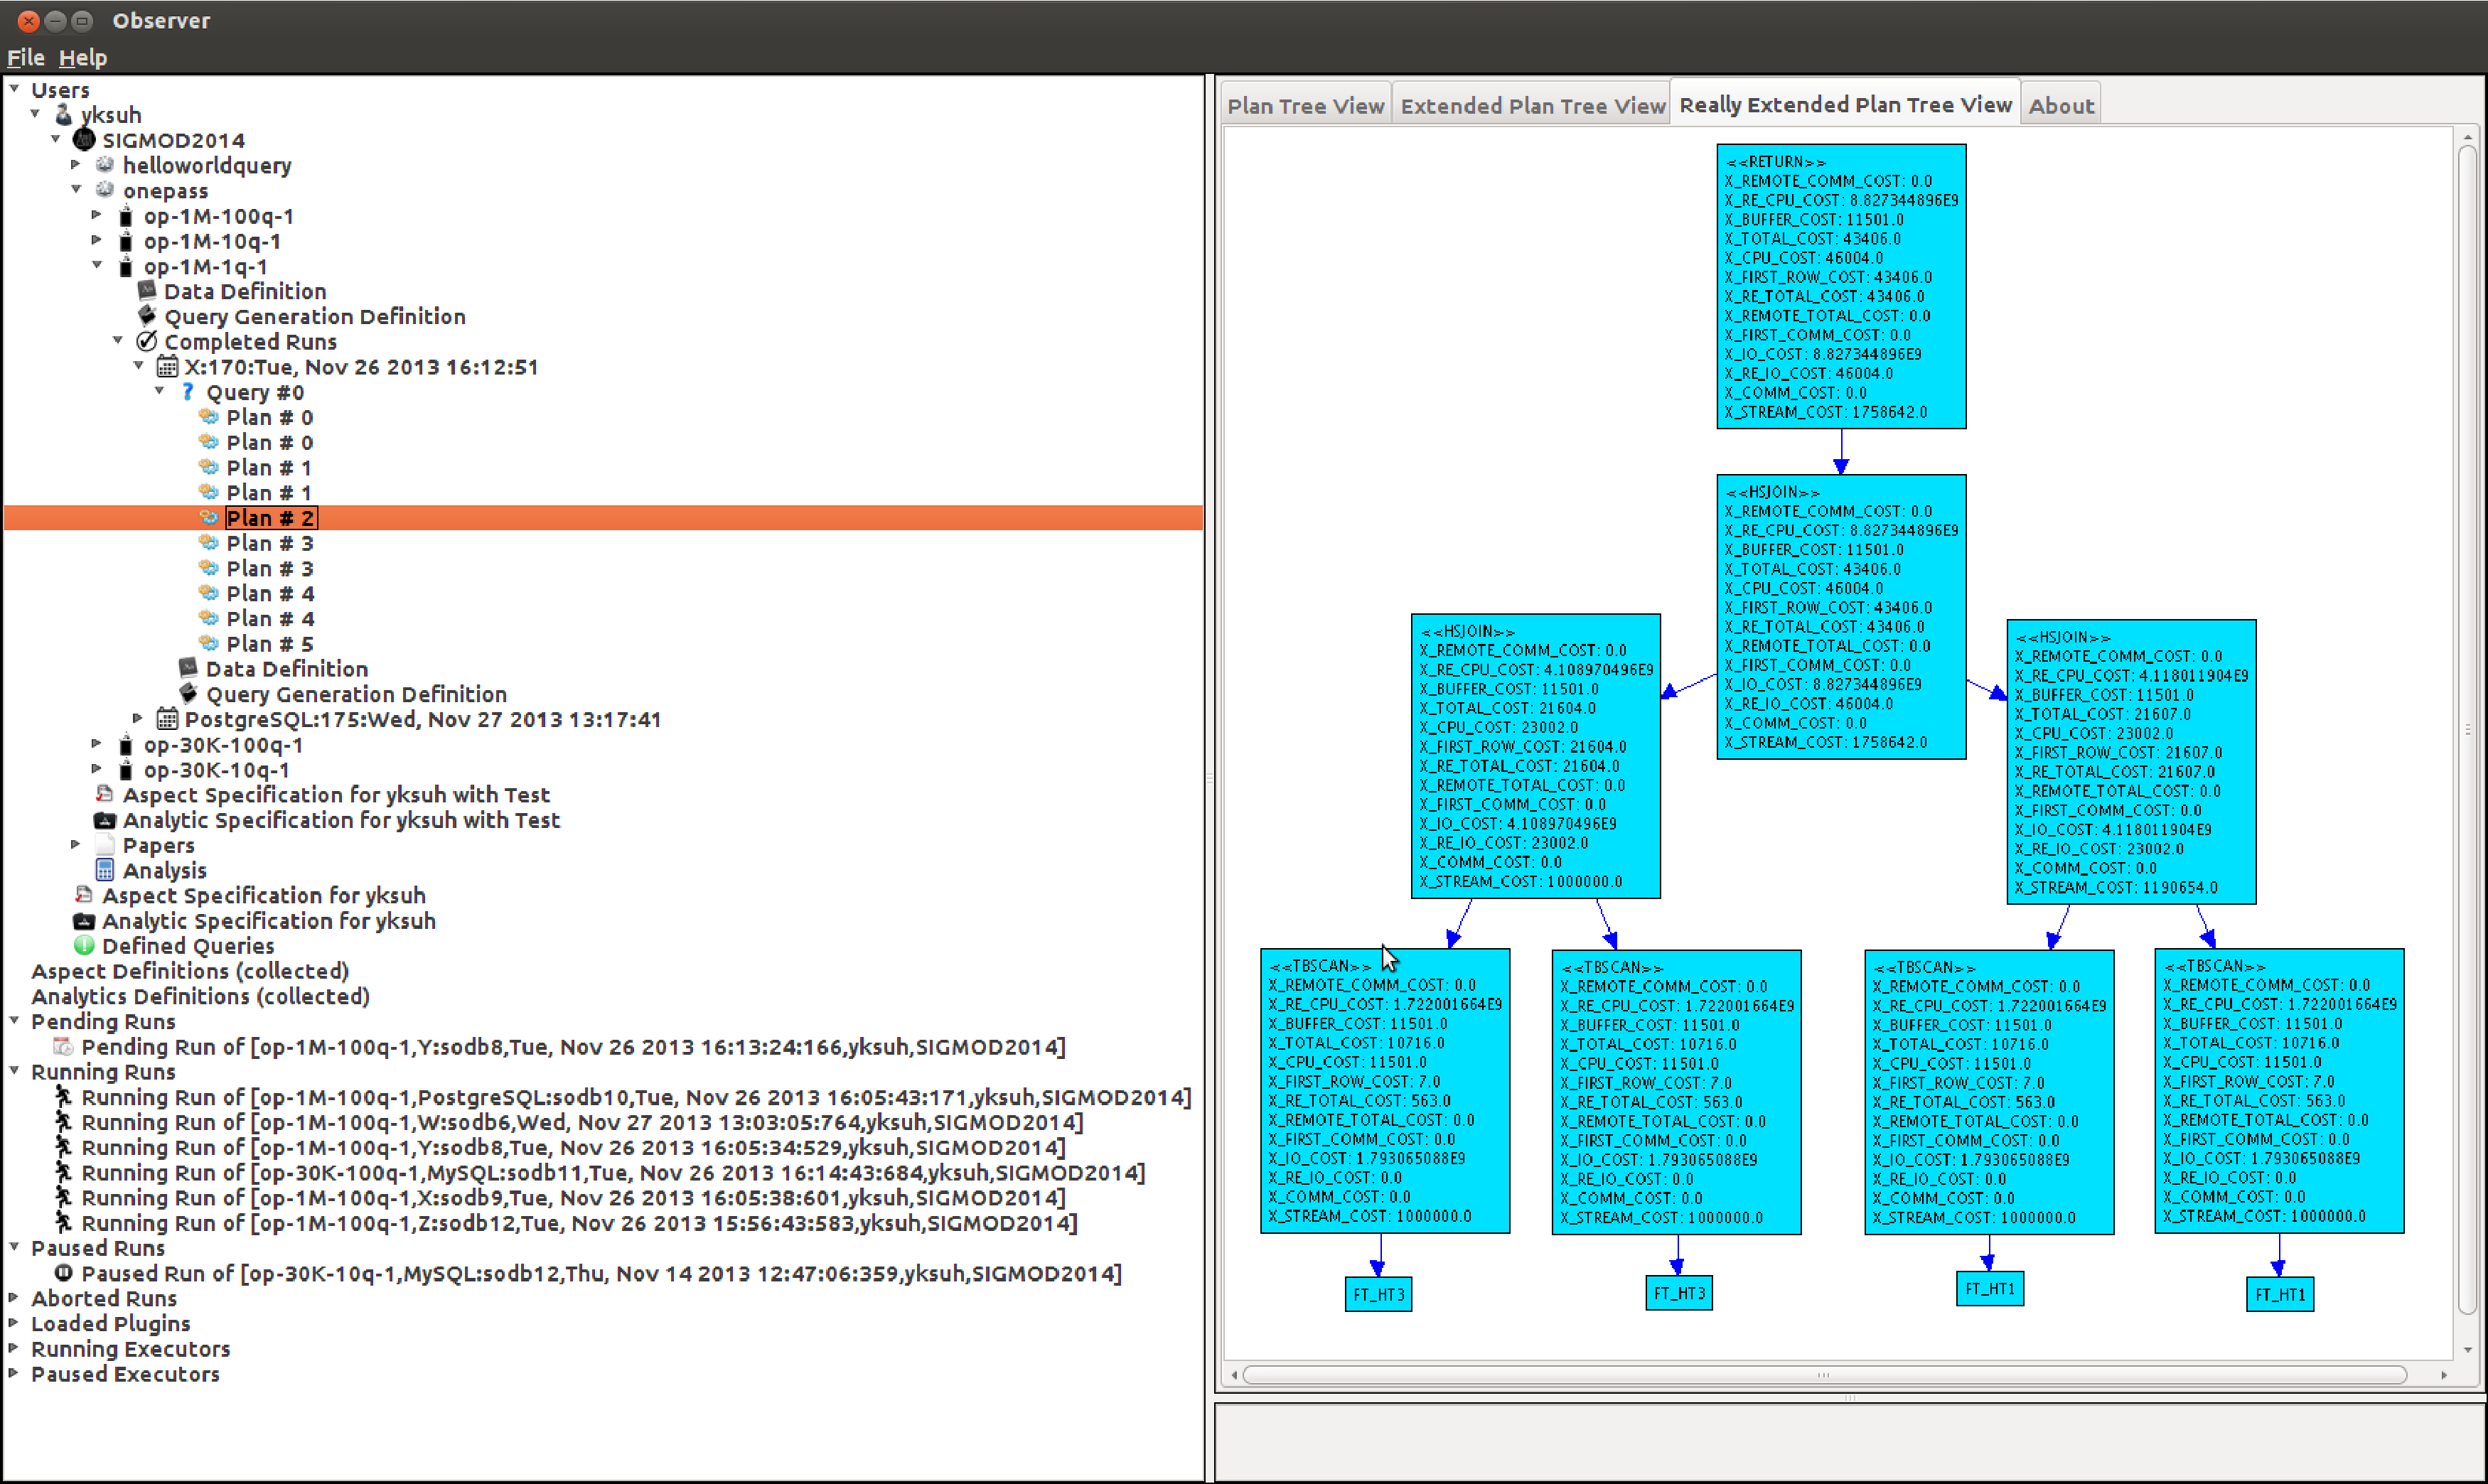
\includegraphics[scale=0.3]{./figures/observer_gui_new}
\caption{$\azdb$ Observer\label{fig:observer_gui}}
\vspace{-0.1in}
\end{figure*}

\subsection{Decentralized Monitoring Schemes}
In this section, we present a variety of novel, decentralized monitoring schemes being in use in $\azdb$.
%These monitoring tools help a user manage and monitor experiments on a remote site.

\subsubsection{Observer}\label{sec:observer}
%Observer provides a database researcher with GUI for loading, scheduling, and running an experiment, and later analyzing 
%the completed experiment results. It is a stand-alone Java application.
Observer is an integrated \hbox{GUI} for \hbox{conducting} experiments involving a large number of queries and \hbox{analyzing} the \hbox{results}. 
The GUI is implemented with Java Swing API. When \linebreak \hbox{launching} \hbox{Observer}, a user can see the main \hbox{GUI} in \hbox{Figure}~\ref{fig:observer_gui}.

%When launching Observer, he is asked to choose a labshelf. 
%Observer then connects to the labshelf server to load and expose to him the data stored in the chosen labshelf.
%The data include a labshelf user(s), notebook(s), experiment(s), pending, running, paused, and aborted experiment run(s), 
%query execution results in the experiment run(s), and executor(s) currently in use.
%An experiment run is an instance of an experiment assigned to a chosen DBMS started at a specific time.

%\begin{figure}[htp!]
%\centering
%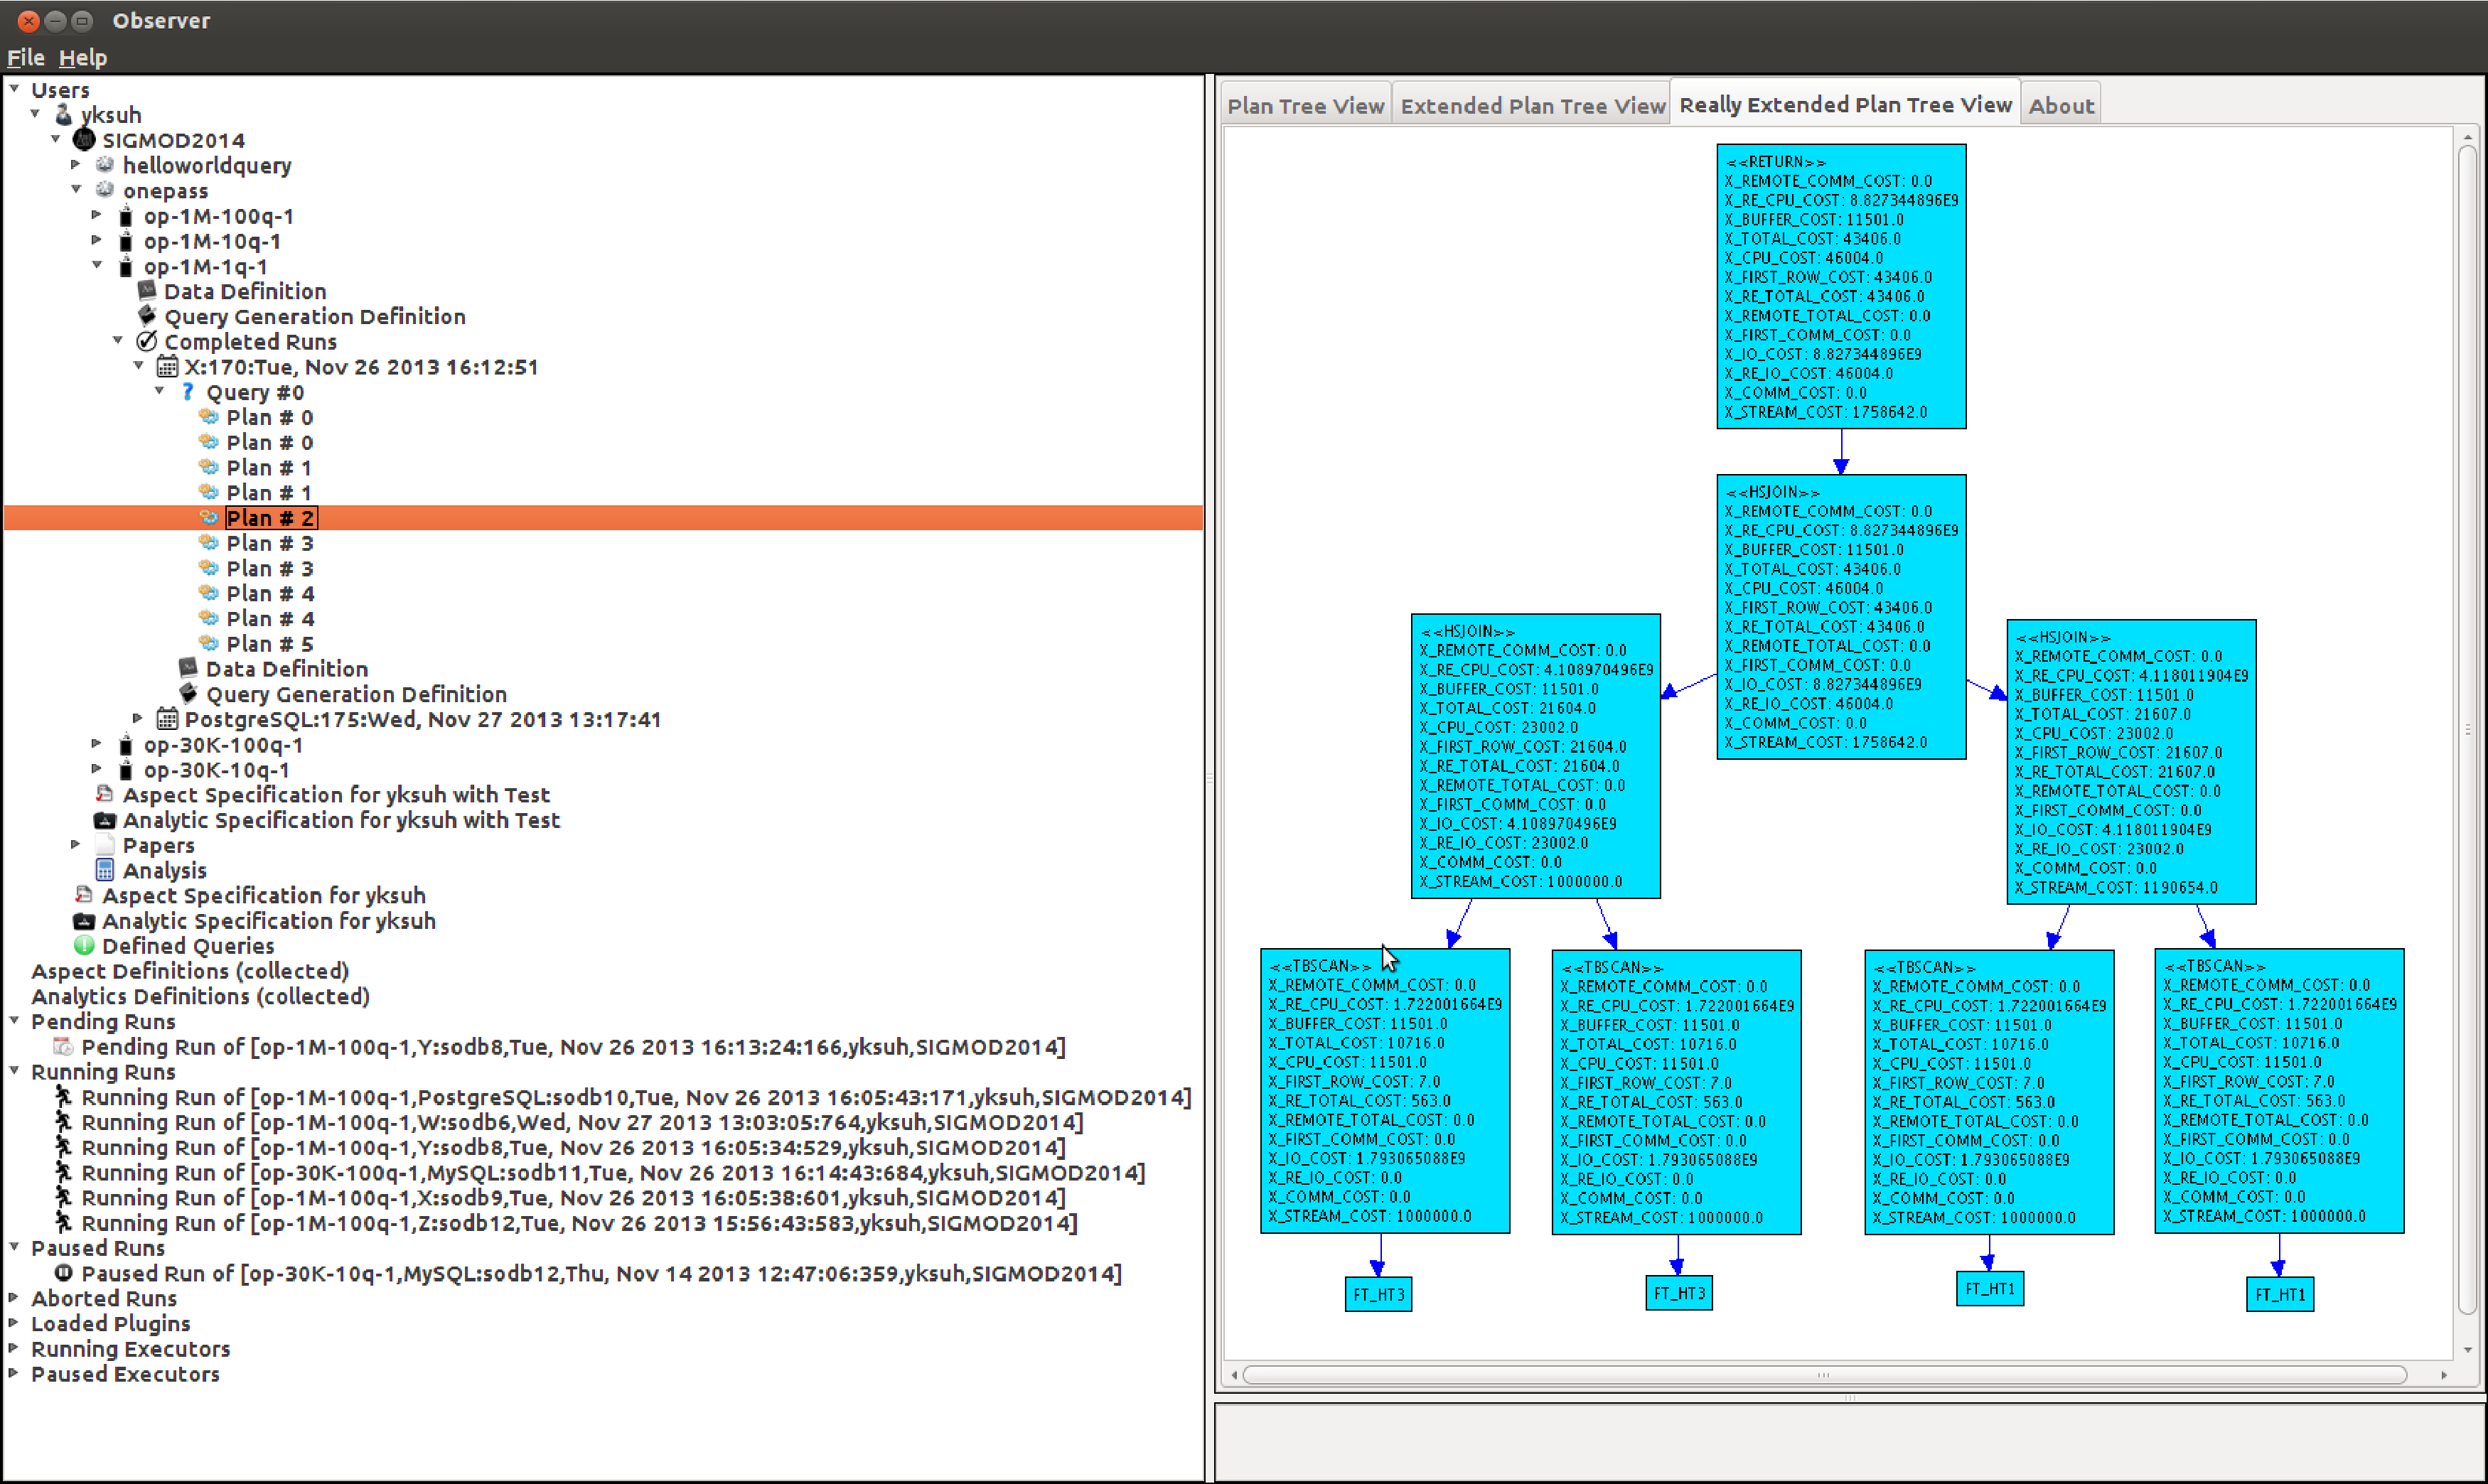
\includegraphics[scale=0.18]{./figures/observer_gui_new}
%\caption{$\azdb$ observer\label{fig:observer_gui}}
%\end{figure}

%For instance, under `{\tt Users}' node, there are two labshelf users, 
%named `{\tt Sabah}' and `{\tt yksuh}', created in the labshelf. 
%User `yksuh' has created `{\tt SIGMOD2014}' notebook, under which 
%there are two experiment scenarios, named `{\tt helloworldquery}' and `{\tt onepass}'.
%A scenario defines what an experiment concerns. 
%For example, in the {\tt onepass} scenario, while varying the cardinalities, 
%if we detect different query plans, we execute the same query at adjacent cardinalities (apart from 10K).}s:`{\tt exhaustive}' and `{\tt onepass}'.

The \hbox{Observer} \hbox{GUI} has a {\em tree-structured} form. 
A left-hand tree node is associated with data \hbox{corresponding} to \hbox{experiment} provenance. 
For instance, `{\tt Users}' node \hbox{contains} users in a labshelf selected by the user. 
In the figure, \hbox{under} the `{\tt Users}' node, we can see a \hbox{labshelf} user (node), named `{\tt yksuh}'\shorten{, 
\hbox{under} which there exists a \hbox{notebook} node, named `{\tt VLDB2014}', which \hbox{represents} a lab \hbox{notebook} on the \hbox{labshelf}}. 
In the right-hand side, more detailed information on a \hbox{chosen} left-hand node is \hbox{provided} in tabbed views. 
For the selected plan node (`{\tt Plan \# 2}') to be discussed shortly, 
the \hbox{corresponding}, expanded plan tree is exhibited with \linebreak \hbox{various} {\em operator-wise} cost estimates, as shown in Figure~\ref{fig:observer_gui}.

%In the figure, for instance, under `{\tt Users}' node, there is one labshelf user, named `{\tt yksuh}', created in the labshelf. 
%User `{\tt yksuh}' has created `{\tt SIGMOD2014}' notebook, under which there are two scenarios, named `{\tt helloworldquery}' and `{\tt onepass}'.
%A scenario defines what an experiment is concerned about and how the experiment should be conducted. 
%For instance, the \linebreak `{\tt onepass}' scenario studies the suboptimality of a set of {\em select}-{\em project}-{\em join} queries 
%on one to four tables, each consisting of four integer columns. 
%Three of the tables are called {\em fixed} tables and have 1M rows each, while 
%the other table is called {\em variable}.
%%In the scenario, while decrementing the cardinality of the variable table from 2M rows to 10K the cardinality of the variable table by 10K, 
%In the scenario, while decrementing the cardinality of the variable table from 2M rows to 10K rows by decrements of 10K, 
%if the plan of a query being studied is changed between adjacent cardinalities of the table, 
%we execute the query at both cardinalities. Later, we check if the execution time at a lower cardinality 
%is greater than that of a higher cardinality, and if so, the query is reported as {\em suboptimal}.

This GUI allows the user to proceed with running a \linebreak {\em scenario-based} \hbox{experiment}. 
A scenario specifies {\em what an \hbox{experiment} is \hbox{concerned} about} and {\em what specific steps should be executed}. 
To run the scenario on $\azdb$, the user first needs to write the corresponding code in Java. 
For example, a \hbox{scenario} source code, called `{\tt onepass}', can be written to study the query \hbox{{\em suboptimality}} \hbox{phenomenon} such that when the \hbox{execution} plans of a query change between two adjacent \hbox{cardinalities} (called a {\em change point}), the actual elapsed time of that query at a lower \hbox{cardinality} is greater than that of a higher \hbox{cardinality}. 
\shorten{\linebreak `{\tt onepass}' is named after our strategy of decrementing the cardinality only in one direction from the maximum to the mininum.)} 
Once the \hbox{scenario} code is ready, it can be brought as a {\em plugin} into $\azdb$. 

%In the running scenario, he can define four tables, each consisting of four integer columns. 
%Three of the tables are called {\em fixed} tables and have 1M rows each, while the other table is called {\em variable} and initially has 2M rows. 
%While decrementing the cardinality of the variable table by 10K, 
%if the plan of a query being studied is changed between adjacent cardinalities of the table, 
%the sceario executes the query at both cardinalities. Later, he can check if the execution time at a lower cardinality 
%is greater than that of a higher cardinality. If so, the query is reported as {\em suboptimal}.

%In Figure~\ref{fig:observer_gui}, under the `{\tt onepass}' scenario on the \hbox{left-hand} side, there are two loaded 
%experiments, named `{\tt op-1M-10q-1}' and `{\tt op-1M-1q-1}', each of which utilizes the same scenario but has different parameters. 
%In the names, we used the convention where `{\tt op}' stands for the `{\tt onepass}' scenario, 
%`{\tt 10q}' or `{\tt 1q}' refers to the number of queries in the experiments, respectively. 
%`{\tt 1M}' denotes the base cardinality of a table used in the experiment. 
%Lastly, `{\tt 1}' indicates the query set number.
%%Under `{\tt Completed Runs}', two {\tt onepass} runs are finished on DBMS {\tt X}\footnote{The license of the commercial system forbids us to disclose it.}. 
%Under `{\tt Completed Runs}', two {\tt onepass} runs have finished on DBMS {\tt X}. 
%While studying query \#0 ({\tt SELECT t0.id3, t1.id2 FROM ft\_HT3 t3, ft\_HT1 t1, ft\_HT3 t2, ft\_HT1 t0  WHERE (t3.id3=t1.id2 AND t1.id2=t2.id1 AND t2.id1 \linebreak =t0.id4}), 
%the scenario reported a total of six change points, and $\azdb$ recorded 
%each query plan and its associated execution time (although not shown in the figure). 
%In the right hand side, we show one of its query plan trees, denoted as `{\tt Plan \# 2}', 
%with each operator's estimates collected from DBMS {\tt X}. 

Besides, the user needs to write and load into $\azdb$ a simple XML experiment specification, which 
contains \linebreak \hbox{scenario} name, schema definition, \hbox{table} population \linebreak \hbox{direction}, query details, etc. 
Figure~\ref{fig:observer_gui} shows several \linebreak \hbox{experiments} such as `{\tt op-1M-1q-1}' under the `{\tt onepass}' node. 

\shorten{the `{\tt onepass}' scenario node under `{\tt VLDB2014}'}
%`{\tt op}' stands for the `{\tt onepass}' scenario. 
%`{\tt 1q}' refer to the number of queries to be run for the experiments. 
%`{\tt 1M}' denotes the base cardinality of tables in the experiments, and 
%`{\tt 1}' indicates a certain query set number. 

The user can then schedule any of these experiments on a specific \hbox{DBMS}. 
This scheduled experiment instance is termed as `{\em experiment run}' and its status is in `{\em pending}'. 
\hbox{Observer} updates its GUI to show the pending run. 

If an \hbox{executor}, to be discussed in Section~\ref{sec:executor}, has any assigned \hbox{pending} run,
the executor starts to execute that pending run, whose status then is updated to `{\em running}'. 
As the run proceeds, the user can monitor the run's \hbox{status} through this GUI\shorten{as well as through 
the other schemes to be described in next sections}. 
Note that the user can also {\em pause} and {\em \hbox{resume}} the \hbox{running} run if necessary. 
Once the run is \linebreak \hbox{completed}, the user can check the experiment results of the run. 
In \hbox{Figure}~\ref{fig:observer_gui}, two completed onepass runs of \hbox{DBMS} {\tt X} and 
\hbox{PostgreSQL} \hbox{DBMS} are illustrated. 
\shorten{Regarding the completed run on \hbox{DBMS} {\tt X}, we can see that an \hbox{executor} stored a total of six change points while running query \#0\shorten{({\tt SELECT t0.id3, t1.id2 FROM ft\_HT3 t3, ft\_HT1 t1, ft\_HT3 t2, ft\_HT1 t0 WHERE (t3.id3=t1.id2 AND t1.id2=t2.id1 AND t2.id1=t0.id4})} over varying \hbox{cardinalities} of {\tt ft\_HT1} table on \hbox{DBMS} {\tt X}. 
Among the observed plans of query \#0, the `{\tt Plan \# 2}' tree is shown in \hbox{Figure}~\ref{fig:observer_gui}.}
\shorten{For each cardinality of change points, the executor recorded the execution plan of query \#0, ran the query, and measured and recorded into $\azdb$ the elapsed time with collected process information (that will be used for further analysis), which is not shown in the figure.}
For another study, we have implemented a new scenario and an analysis plugin to observe a totally separate 
phenomenon, thrashing~\cite{Thomasian93}. 

%
%In addition, under `{\tt Running Runs}' nodes on the left-hand side of the figure, 
%we can monitor the six runs concurrently executing on \hbox{DBMSes} {\tt X}, {\tt Y}, {\tt Z}, and {\tt W} 
%on machines {\tt sodb6}, {\tt sodb8}, {\tt sodb9}, and {\tt sodb12}, as well as PostgreSQL and MySQL on machines {\tt sodb10} and {\tt sodb11}. 
%($\azdb$ disallows more than two runs to be running at a time on any one physical machine.) 
%Also, under `{\tt Paused Runs}' node, there is one run paused on MySQL on machines {\tt sodb12}. 
%Lastly, the GUI shows aborted runs, loaded various plugins, running executors, and paused executors, if any.

%Assume that the login user created a labshelf user (`Young-Kyoon'). 
%The labshelf user has a notebook (`SIGMOD$\_$2014'), under which he has run the two experiment {\em scenario}
%\footnote{A scenario directs how an experiment on a DBMS should be conducted. 
%The experiment contains a set of SPJ queries concerning from one to four tables, each 
%consisting of four integer columns. 
%One of the tables is called {\em variable} table,
%which is initially populated with two times more rows than the specified cardinality (e.g., 30K) 
%and incrementally decreased at a certain granularity (20K). 
%The other ones called {\em fixed} one, which has its fixed cardinality (e.g., 30K). 
%In the {\tt exhaustive} scenario each query is run at every cardinality while varying the cardinality of 
%the variable table (i.e. 60K) at the granularity. 
%In the {\tt onepass} scenario, while varying the cardinalities, 
%if we detect different query plans, we execute the same query at adjacent cardinalities (apart from 10K).}s:`{\tt exhaustive}' and `{\tt onepass}'. 
%Due to lack of space, Figure~\ref{fig:observer_gui} shows only the completed {\tt exhaustive} experiment (named `eh-30K-2q-1') 
%run of 2 queries on Microsoft SQL Server. 
%Specifically, in the right-hand side the query 1's plan tree is shown when the variable table's cardinality was 40K; 
%in the query plan tree, we can see each query operators' estimates as well. 
%In addition, under `Running Runs' nodes, we can monitor the five experiment runs currently running on each different DBMS, 
%and under `Paused/Aborted Runs' nodes, we can also see one run paused on IBM DB2, and two aborted runs on MySQL and oracle, respectively. 
%
%`Loaded Plugins' shows different type of plugins used in $\azdb$. 
%`Experiment Subject Plugins' represents different DBMSes, treated as {\em experiment subject}, 
%`Scenario Plugins' node includes different experiment scenarios, and lastly, 
%`Evaluation Plugins' node contains a variety of evaluation plugins for further analysis of completed runs. 
%
%Finally, `Executors' node shows different executors running on the same machine where a DBMS gets installed. 
%We will shortly discuss executors in more details.

%\subsubsection{Web Application - Ajax}
\subsubsection{Web Apps}
$\azdb$ also provides a web app using Ajax~\cite{ajax}. 
A user can access the web app running on an $\azdb$ web server 
and make a request through a web browser. 
The web app then invokes an \hbox{AjaxManager} (a Java class), 
which interacts with the \hbox{labshelf} DBMS server to pull the requested data in a labshelf.
The server then responds to the user with the data.
%Finally, the page will be dynamically updated to display the received data as done in the Observer GUI. 
%In this way, a user can launch new experiments and subsequently monitor how they are going through the web application. 
%Due to lack of space, we do not show its snapshot, but the audience will be able to 
%watch experiment runs through Ajax application. 
The web app \hbox{provides} the same functionalities and GUI as \hbox{Observer}, 
without requiring direct access to the labshelf server, thereby achieving greater security.
%achieving greater security\shorten{, 
%without requiring direct access to the labshelf DBMS server, thereby achieving greater security}.

\subsubsection{Mobile Apps}
%\todo{Ask Ben.} 
To more flexibly monitor the executing runs we also make mobile apps available for the user.
\shorten{is also available for a user.}
We have built the mobile apps on both \hbox{Android} and \hbox{iOS}. 

The mobile apps provide simple functionalities, compared to \hbox{Observer}. 
%The \hbox{functionalities} of the apps are simpler than those of \hbox{Observer}. 
The user cannot conduct query execution data \hbox{analysis} through the mobile apps, 
but the user can set up a convenient \hbox{monitoring} environment on the mobile apps.

%The user can select a \hbox{labshelf} and view \hbox{currently} \hbox{pending}, running, and paused runs, 
%as well as \hbox{executors} \hbox{being} used for the labshelf, via the apps. 

The mobile apps also make a request to the same \linebreak 
$\azdb$ web server, 
which invokes methods from \linebreak \hbox{AjaxManager}. 
As mentioned earlier, \hbox{AjaxManager} then connects to the labshelf server and 
retrieves the data \linebreak \hbox{corresponding} to the user's request regarding 
user \hbox{logins}, and \hbox{experiment} and \hbox{executor} \hbox{statuses}. 

% via an \hbox{API} written in \hbox{JSP} and \hbox{Java}
 
%The mobile apps through the web server can connect to the same labshelf DBMS server as used in \hbox{Observer}, 
%to retrieve \hbox{information} about user \hbox{logins}, \hbox{experiment} and \hbox{executor} \hbox{statuses}. 

%To respond to the user's request, 
%the corresponding \hbox{AjaxManager}'s method is invoked to \hbox{retrieve} \hbox{information} about user 
%\hbox{logins}, \hbox{experiment} and \hbox{executor} \hbox{statuses}.
%However, the apps allow the user to select a labshelf and view \hbox{currently} pending, running, and paused runs 
%as well as \hbox{executors} \hbox{being} used for this labshelf. 
%which in turn calls methods from \hbox{AjaxManager} to \hbox{retrieve} \hbox{information} about user 
%\hbox{logins}, \hbox{experiment} and \hbox{executor} \hbox{statuses}. 
%Communication happens with the server via \texttt{GET} and \texttt{PUT} \texttt{http} requests.

\begin{figure}[htp!]
	\centering
	\subfigure[Main]{
		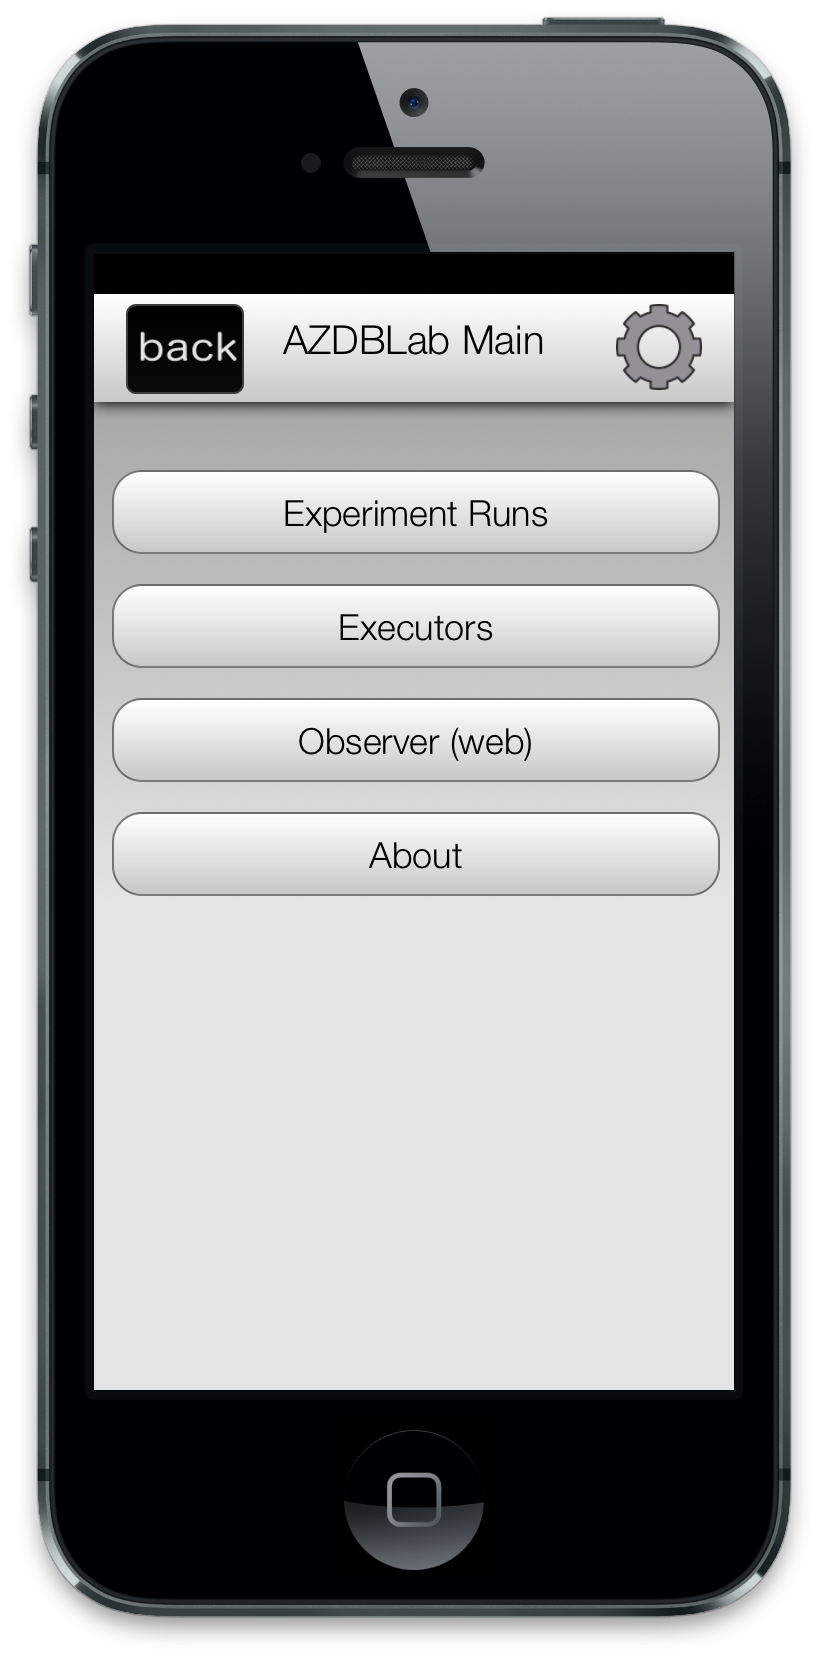
\includegraphics[scale=0.17]{./figures/main}
		\label{fig:main}
	}
	\subfigure[Exp. Runs]{
		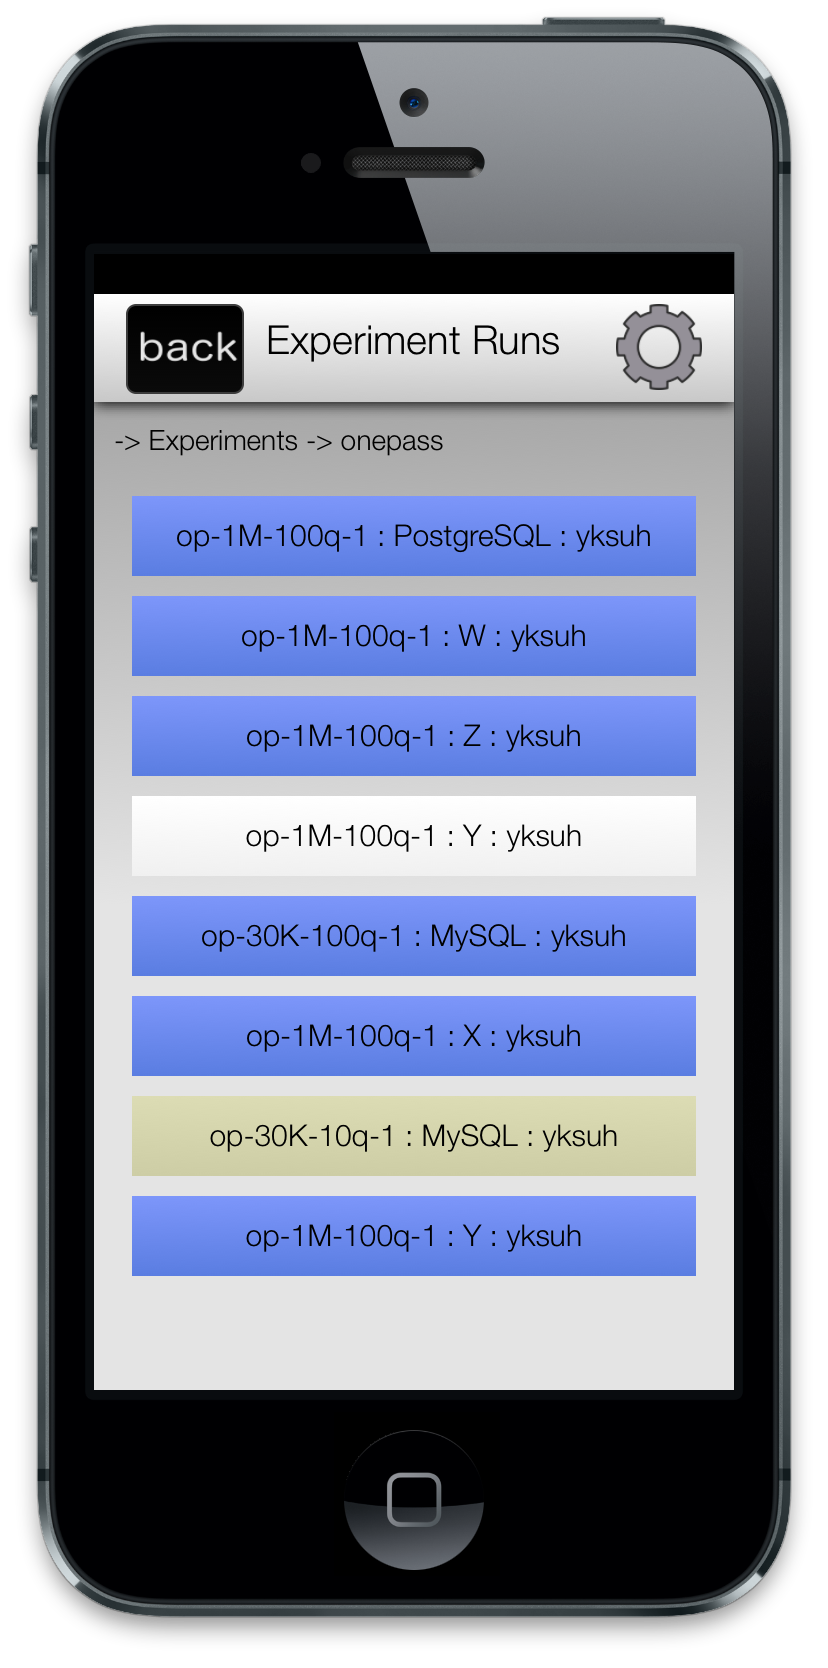
\includegraphics[scale=0.17]{./figures/experiment_run}
		\label{fig:exp_runs}
	}
	\subfigure[A running run]{
		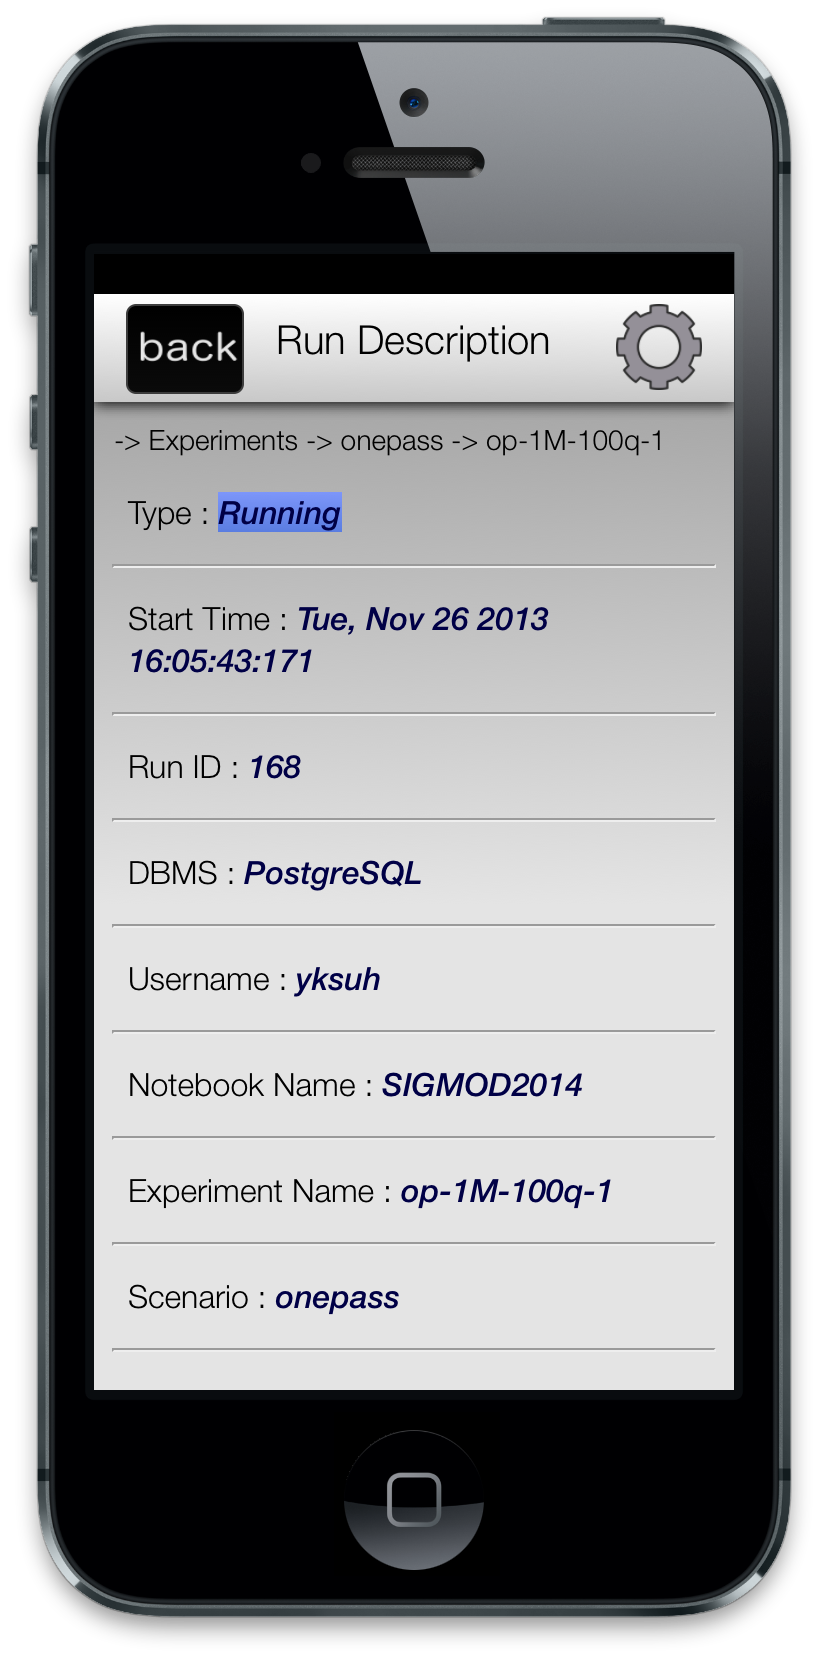
\includegraphics[scale=0.17]{./figures/run_description}
		\label{fig:exp_details}
	}
	\vspace{-0.1in}
	\caption{$\azdb$ mobile app\label{fig:mobile_app}}
	%\vspace{-0.1in}
\end{figure}

Figure~\ref{fig:mobile_app} illustrates the $\azdb$ mobile (iOS) app. \linebreak
When a user starts the mobile app, the user is presented with a login screen, into which the user's credentials must be provided. 
%The credentials are validated through the JSP API. 
%User logins are stored on the server in XML files (one per user login) 
%that contains the user name, password hash, and superuser status.
Once the credentials are validated, the user can see the main screen consisting of four menus, as shown in \hbox{Figure}~\ref{fig:main}. 
`{\tt Experiment Runs}' lists all the runs in a \hbox{chosen} labshelf, as illustrated in \hbox{Figure}~\ref{fig:exp_runs}. 
%(The runs are the ones as shown in Figure~\ref{fig:observer_gui}.)
An item in blue \hbox{indicates} a currently running run, one in white a \hbox{pending} run, and one in gray a paused run. 
%To get a full list of information about an experiment, he can choose one from the list, 
%and a full detail of the experiment will be brought up as a new page, as illustrated in Figure~\ref{fig:exp_details}. 
A running run on \hbox{PostreSQL} is exhibited in Figure~\ref{fig:exp_details}.
%This browsing and viewing process is essentially the same for viewing executors. 
The `{\tt Executors}' menu provides currently running \hbox{executors}, the `{\tt Observer}' menu shows 
the same view as the web app's one, and the `{\tt About}' menu provides a description of $\azdb$. 

%In order to allow this application to run on multiple mobile OSs with minimal effort, 
%we built it using the PhoneGap development library. Using PhoneGap, 
%we were able to write the majority of the software using platform-agnostic web standards 
%such as HTML and CSS for the UI and Javascript and JQuery for the networking and other general logic. 
%We have tested the application on both iOS and Android, 
%and we plan on testing in on the Windows Phone OS in the future.

%\subsubsection{Watcher}
%%\todo{Ask Jen.}
%Watcher is a utility program used for watching an executor's behaviors during an experiment. 
%It frees a user from keeping an eye at all times on how the experiment goes. 
%Watcher immediately sends a user via email the notification messages when we encounter the following situations 
%where 1) an executor gets stopped, 2) a DBMS unexpectedly shuts down, 3) a running experiment gets paused by an exception, and 
%4) the labshelf server is not responsive. 

%Watcher sends a user the notification via his email, so that the user can go to the terminal of the machine and 
%fix the problem. Currently, it reports 

\subsection{Executor}\label{sec:executor}
%An executor is a stand-alone \hbox{Java} \hbox{application} 
%and \hbox{conducts} an experiment on a \hbox{DBMS}, which is co-located with the \hbox{executor}, as illustrated in Figure~\ref{fig:azdblab_arch}. 
%It is a stand-alone Java application as observer, and it works with a chosen experiment subject plugin.
%The executor utilizes a \hbox{DBMS} experiment \hbox{subject} plugin. 
An executor \hbox{conducts} an experiment on a co-located \linebreak \hbox{DBMS}, as illustrated in Figure~\ref{fig:azdblab_arch}. 
The executor is a stand-alone Java application, utilizing a \hbox{DBMS} experiment \hbox{subject} plugin. 
A user can launch an executor and schedule a \linebreak \hbox{pending} run to the executor. 
The executor can begin the \hbox{experiment} by \hbox{loading} the run's scenario and experiment subject \hbox{plugins}. 
The \hbox{executor} then creates and populates tables, executes queries, records QE results into $\azdb$, and finishes the run, 
as explained in \hbox{Section~\ref{sec:observer}}. 
If any \hbox{exception} occurs during the \hbox{experiment}, the executor can pause the run. Later, the user can unpause the run. 
\hbox{Multiple} executors can be in action, perhaps using distinct instances of the same \hbox{DBMS}, 
each on a different \hbox{machine}. 
To avoid \linebreak \hbox{undesirable} latency by network traffic, we ensure that the executor must run on the same machine hosting a \hbox{DBMS}. 
%measures query time, and records into $\azdb$ the measured time with collected process information. 

%When the researcher launches an executor, the executor interacts with the labshelf server every five seconds, 
%to check if there is any pending experiment run assigned to the executor as mentioned in Section~\ref{fig:observer_gui}. 
%If so, the executor starts the experiment; it loads necessary plugins like onepass scenario or experiment subject, 
%creates and populates tables along with the experiment specification, executes a query on the tables, 
%measures query time, and records into $\azdb$ the measured time with collected process information. 
%During the experiment, if the executor encounters any exception occurs, the executor will pause the ongoing experiment run. 

%\vspace\fill

\section{Demonstration}\label{sec:demo_overview} 
Our demo consists of two parts: 1) running experiments with hundreds of queries on different \hbox{DBMSes} and 2) then analyzing QE 
results from the completed runs. 
%We describe what steps the audience will do.

%\subsection{Running an experiment}
%The goal of this demonstration is to show how an experiment can be run and managed in $\azdb$. 
The goal of the first part of this demo is to show how a database \hbox{researcher} can schedule and run a large-scale experiment in $\azdb$. 
The steps are as follows.

%\pagebreak

{\bf Step 1}: An auditor launches \hbox{Observer} and selects a \linebreak \hbox{labshelf}. 
The user then creates a \hbox{labshelf} user and the user's lab notebook. 
In turn, the user loads into the user's \hbox{notebook} an XML experiment specification guiding table population and referring to queries. 

{\bf Step 2}: The user selects a \hbox{DBMS}, schedules a run of the \hbox{experiment} on the \hbox{DBMS} and then launches an executor for that DBMS. 
After that, the user can see on console that the experiment gets started on the DBMS. 
The user may add other \hbox{DBMSes} in order to run the same experiment.

{\bf Step 3}: The user monitors the run's status via \hbox{Observer} (or the \hbox{iOS} app). At the end, the user will see the run done. 

%\subsection{Analyzing experiment results}
In the second part of this demo, the audience will see how the user can conduct a study on the completed runs. %Here are the demo steps:

{\bf Step 4}: The user creates a {\em paper} under her notebook and the study under that paper in the \hbox{Observer} \hbox{GUI}.

{\bf Step 5}: For the study, the user chooses the completed runs via dialog box and 
executes \hbox{Tucson} \hbox{Timing} \hbox{Protocol} (\hbox{TTP}) on the runs. 
The automated protocol performs a \hbox{series} of {\em sanity checks} on QEs of the runs, shows \hbox{validation} results, and calculates query time on the passed QEs. 

%{\bf Step 3}: The user finally produces a paper based on the analyzed results. 
{\bf Step 6}: The user finally produces a \hbox{PDF} document \linebreak \hbox{containing} the protocol analysis results. 
The user can also \hbox{create} graphs showing the estimated costs of a plan operator (e.g., hash join) over increasing cardinalities. 
The analysis results and graphs can be used for producing the paper.

\shorten{In this demo, the audience will see the comprehensive provenance of the data used by, and generated for a study.} 
\shorten{Thanks to this feature, a researcher does not have to worry about the data source of the graphs or tables included in the study.}
%For instance, a graph can be included in a paper, but one may not know where its data source come from. 
%$\azdb$ keeps every provenance of where data comes
%
%The data source of the graphs can be found in $\azdb$, so that a user does not have to worry about where 
%his data come from. 

%In general, the analysis on the experiment runs can include graphs. $\azdb$ helps link a specific study 
%to 
%Since $\azdb$ stores 
%This demo will show how seamlessly $\azdb$ manages provenance of data used in an analysis for a paper. 
%the provenance of where data come from, 
%
% concerns multiple experiment runs. From these runs 
%The graphs are generated based on the data obtained through experiment runs. 
%
%used for a paper.
%
%The graphs will visualize the estimated cost of a chosen plan operator 
%(like hash join) over increasing cardinality. 
%
%In general, 
\shorten{
\section{Summary}\label{sec:summary}
In this demo, we present $\azdb$, a {\em DBMS-oriented} lab for large-scale empirical studies across multiple \hbox{DBMSes}. 
\shorten{$\azdb$ gives database researchers full \hbox{support} for managing a large-scale experiment with hundreds of queries and automatically analyzing and visualizing the query execution results.}
\shorten{$\azdb$ allows database researchers to run experiments simultaneously on the \hbox{DBMSes} and 
%automatically collects all data provenance regarding the experiments for further analysis. 
automatically collect all provenance regarding the experiments for further analysis. 
Our demo presents the audience with an actual experiment scenario on \hbox{DBMSes} running on our dedicated machines 
%and shows the audience how the experiment can be monitored, and then the results can be analyzed in $\azdb$. 
and shows the audience how the experiment can be monitored and the results can be analyzed in $\azdb$.}
}

%\vspace{-0.3ex}
\vspace{-1.2ex}

\section{Acknowledgement}
We thank to T.~Buchanan, S.~Currim, B.~Dicken, \linebreak M.~\hbox{Johnson}, P.~Kaslo, A.~Kvochko, T.~Lowry, 
H.~Zuniga, and others for their contributions to $\azdb$.

\vspace{-0.9ex}
%\vspace{\vfill{*}}

\bibliographystyle{abbrv}
\newcommand{\etalchar}[1]{$^{#1}$}
%{\small
\begin{thebibliography}{99}
\vspace{0.1em}
\bibitem
{ajax}
W3C, ``XMLHttpRequest'', January 2014.

\bibitem
{ergalics}
R. T. Snodgrass, “Database Ergalics”, \url{http://cs.}\linebreak\url{arizona.edu/~rts/ergalics}, viewed Mar 28, 2014.

\bibitem
{Currim}
S.~Currim, R. T. Snodgrass, Y-K. Suh, R.~Zhang, M.~Johnson, and C.~Yi, ``DBMS Metrology: Measuring Query Time,'' in {\em SIGMOD}, 
pp.~261--272, 2013.

%\bibitem
%{Currim2}
%S.~Currim, et. al., ``A Causal Model of DBMS Suboptimality,'' in {\em Proceedings of the ACM SIGMOD conference},
%In submission, 2014.

\bibitem
{WA05MoteLab}
G.~Werner-Allen, P.~Swieskowski, and M.~Welsh, ``MoteLab: A Wireless Sensor Network Testbed,'' in {\em IPSN}, pp.~483--488, 2005.
%
\shorten{\bibitem
{Nandugudi13PhoneLab}
A.~Nandugudi, A.~Maiti, T.~Ki, F.~Bulut, M.~Demirbas, T.~Kosar, C.~Qiao, S.~Y.~Ko, and G.~Challen, ``PhoneLab: A Large Programmable Smartphone Testbed,'' in {\em SENSEMINE}, pp.~1--6, 2013.}
%
\bibitem
{Larkou13SmartLab}
G.~Larkou, C.~Costa, P.~G.~Andreou, A.~Konstantinidis, and D.~Zeinalipour-Yazti, ``Managing Smartphone Testbeds with SmartLab,'' in {\em LISA}, pp.~115--132, 2013.
%
\bibitem
{Peterson2006planetlab}
L.~Peterson, A.~Bavier, M.~E.~Fiuczynski, and S.~Muir, ``Experiences Building PlanetLab,'' in {\em OSDI}, pp.~351--366, 2006.
%
\bibitem
{cuervo2011crowdlab}
E.~Cuervo, P.~Gilbert, B.~Wu, and O.~P.~Cox, ``\hbox{Crowdlab:} An Architecture for Volunteer Mobile Testbeds,'' in {\em COMSNETS}, pp.~1--10, 2011.
%
\bibitem
{Ram}
S.~Ram and J.~Liu, ``Understanding the Semantics of Data Provenance to Support Active Conceptual Modeling,'' in {\em ACML}, pp.~1--12, 2006.
%
\bibitem 
{Snodgrass99}
R. T. Snodgrass, {\bf Developing Time-Oriented Database Applications in SQL}, \shorten{Morgan 
Kaufmann Publishers, Inc., San Francisco, CA,} July 1999\shorten{, 504+xxiv pages}.
%
\bibitem
{Reddy05}
R.~Naveen and J.~R.~Haritsa, ``Analyzing Plan Diagrams of Database Query Optimizers,'' in {\em VLDB}, 
pp.~1228--1239, 2005.

\bibitem
{Thomasian93}
A.~Thomasian, ``Two-Phase Locking Performance and Its Thrashing Behavior,'' in {\em ACM TODS}, 
pp.~579--625, 1993.

\end{thebibliography}
%}
\end{document}
